\subsection{Victoria Park Dataset}
\subsubsection{Computational Performance of EKF-SLAM}
EKF-SLAM has been critizised for a variety of reasons in the literature, and one of the issues often brought up is computational performance as the map grows. Keeping the computation time down is of paramount importance in the online SLAM problem where delayed updates are not acceptable. In fact, each timestep of EKF-SLAM has a computational complexity of $\mathcal{O}(n^2)$ in the number of detected landmarks\cite{divideandconq}, something our implementation confirms. When tuned to provoke lots of landmark detections (around 800), the update step of the Kalman filter takes quadratic time, as shown in figure \ref{fig:update_time_landmarks}. These results show that in large environments, EKF-SLAM alone fails to meet the time-requirements for online SLAM.
\begin{figure}[H]
\centering
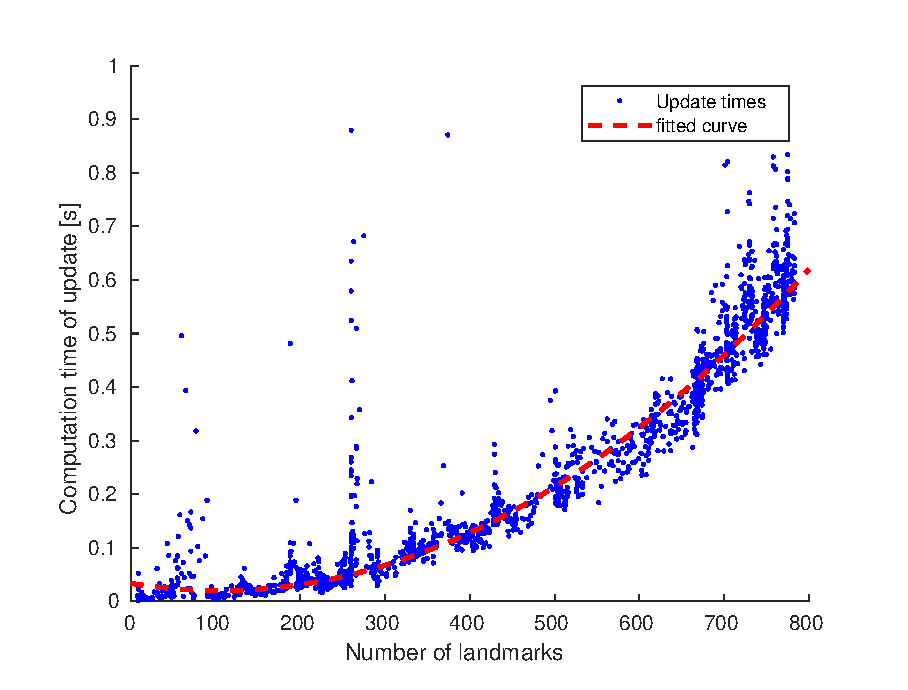
\includegraphics[width=0.7\textwidth]{plots/a3/update-time-vs-landmarks}
\caption{Update time vs landmarks}
\label{fig:update_time_landmarks}
\end{figure}


